\documentclass[conference]{IEEEtran}

\usepackage{graphicx}
\usepackage{amsmath}
\usepackage{hyperref} % still needed

\title{Project Delivery 3}

\author{
\IEEEauthorblockN{Joshua Thomas}
\IEEEauthorblockA{
MS in Artificial Intelligence Systems\\
University of Florida\\
Gainesville, USA\\
joshuathomas@ufl.edu}
}

\begin{document}

\maketitle

\section{Project Summary}

This project aims to develop a binary audio spoofing detection system that classifies speech recordings as either bonafide (real) or spoofed (AI-generated). The motivation for this work arises from the rapid advancement and accessibility of speech synthesis and voice cloning technologies, which introduce significant security and reliability concerns in applications such as voice-based authentication, fraud detection, and digital media integrity.

Since Deliverable 1, substantial progress has been made in building a complete end-to-end machine learning pipeline. The ASVspoof 2019 dataset has been fully integrated, and a robust data loading module has been implemented to parse protocol files, extract labels, and associate each audio sample with its corresponding spoofing system. A preprocessing pipeline has been developed to standardize waveform inputs through normalization and fixed-length adjustment, and audio signals are transformed into mel spectrogram representations to enable effective feature extraction.

Building on this foundation, a baseline convolutional neural network (CNN) model has been implemented, trained, and evaluated. Initial experiments using standard dataset splits resulted in very high classification accuracy, but further analysis revealed that this performance was misleading due to the model being evaluated on spoofing systems it had already seen during training. To address this limitation, the data pipeline was refined to support system-based filtering, allowing for controlled experiments where the model is trained on a subset of spoofing systems and evaluated on unseen ones.

This refinement is critical, as it shifts the focus from simple classification accuracy to true generalization—the ability to detect novel spoofing methods. By restructuring the dataset in this way, the project now more accurately reflects real-world deployment conditions, where new spoofing techniques continuously emerge. Preliminary results from these experiments indicate a significant drop in performance when evaluating on unseen systems, highlighting the limitations of the baseline CNN and motivating the need for more advanced approaches.

Remaining work includes refining evaluation metrics such as Equal Error Rate (EER), improving model robustness, and implementing more advanced architectures such as Wav2Vec2 or HuBERT to enhance generalization performance. Additionally, an interactive interface will be developed to demonstrate the system’s capabilities.

\section{System Architecture and Pipeline}

The system is designed as a modular pipeline that processes
raw audio inputs and produces a classification output indicating
whether the audio is bonafide (real) or spoofed. Each stage of
the pipeline transforms the data into progressively more structured
representations suitable for machine learning.

Compared to Deliverable 2, the architecture has been refined
to include a dedicated data loading and system filtering stage,
as well as a complete training and evaluation pipeline. These
additions enable controlled experimentation and more realistic
performance assessment on unseen spoofing techniques.

The overall structure of the system is shown below.

\begin{figure}[htbp]
    \centering
    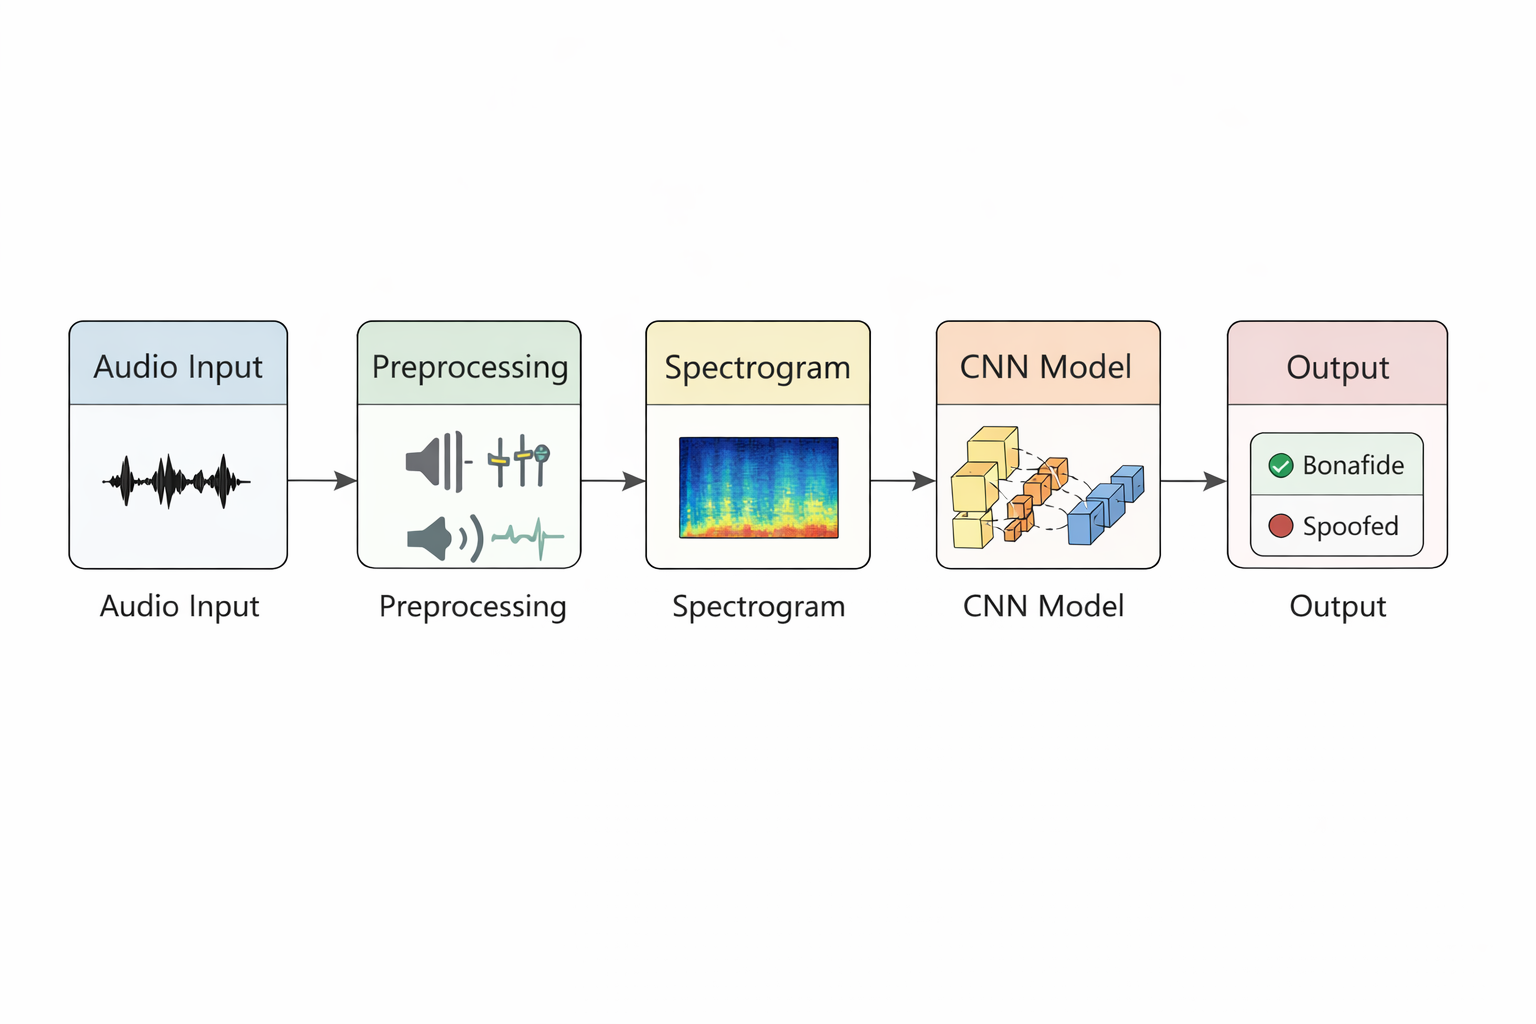
\includegraphics[width=0.45\textwidth]{Audio spoofing detection pipeline diagram.png}
    \caption{System architecture for audio spoofing detection pipeline}
    \label{fig:your_label}
\end{figure}


Audio data is first loaded from the ASVspoof 2019 dataset,
which contains both bonafide and spoofed speech samples.
These samples serve as the input to the system and vary in
length, quality, and recording conditions.

\subsection{Data Loading and System Filtering}

Audio data is loaded from the ASVspoof 2019 dataset, which
contains both bonafide and spoofed speech samples generated
using multiple spoofing systems (e.g., A01–A19). In addition
to mapping each audio file to its corresponding label, the data
loader parses protocol files to extract the spoofing system
associated with each sample.

A key refinement introduced in this stage is system-based
filtering, which allows the dataset to be partitioned based on
spoofing techniques rather than predefined dataset splits. This
enables experiments where the model is trained on a subset of
spoofing systems and evaluated on unseen ones.

This modification is critical for evaluating generalization,
as it more accurately reflects real-world deployment scenarios
where new spoofing methods may not have been encountered
during training.

\subsection{Data Pre-processing}

During pre-processing, each waveform undergoes normalization
and length standardization through padding or truncation.
Since audio samples in the dataset have different durations,
it is necessary to enforce a fixed input length so that batches can be processed efficiently during training. Shorter samples
are padded with zeros, while longer samples are truncated to
a predefined length.

In addition to length normalization, waveform amplitudes
are scaled to a consistent range. This helps stabilize training by
reducing variation in input magnitude across different samples.
Without this step, large amplitude differences could negatively
impact the learning process.

The pre-processing stage plays a critical role in ensuring
robustness and stability. Raw audio signals vary in duration,
amplitude, and recording conditions, which can negatively
affect model performance if not addressed. By enforcing a
fixed-length representation, the system ensures uniformity and
prevents shape mismatches during training.

Following pre-processing, each waveform is converted into a
mel spectrogram, which serves as the primary feature representation
for the model. This transformation converts the one-dimensional
time-domain signal into a two-dimensional time frequency
representation. The mel scale approximates human
auditory perception, emphasizing frequencies that are more
relevant for speech processing.

This representation allows the model to capture spectral
patterns and artifacts that may differentiate real and synthetic
speech. For example, spoofed audio may exhibit subtle inconsistencies
in frequency distribution or temporal structure that
are not easily observable in the raw waveform.

This pre-processing pipeline ensures that all inputs are consistent
and compatible with batch-based training while preserving
relevant acoustic characteristics necessary for downstream
classification.

\subsection{Model Processing}

The model component consists of a convolutional neural
network designed to process spectrogram inputs. 

\begin{figure}[htbp]
    \centering
    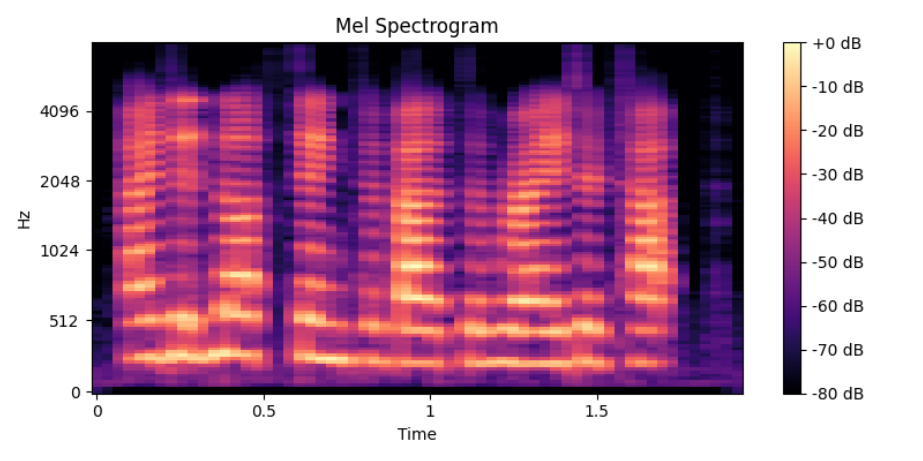
\includegraphics[width=0.45\textwidth]{Mel Spectrogram.png}
    \caption{Example mel spectrogram used as input to the model}
    \label{fig:your_label}
\end{figure}

Convolutional layers extract spatial features from the spectrogram by applying learned filters across the time and frequency dimensions. These filters enable the model to detect patterns associated with real or spoofed speech.

Pooling layers are used to reduce the spatial dimensions
of the feature maps, improving computational efficiency and
helping the model focus on the most relevant features. After
feature extraction, the output is passed through fully connected
layers that produce a binary classification output indicating
whether the input audio is bonafide or spoofed.

\subsection{Interface Design}

A user interface component is planned for future development.
This interface will allow users to upload audio files,
visualize input signals, and receive predictions along with
confidence scores. The goal is to provide a simple and intuitive
way for users to interact with the system without requiring
technical knowledge.

One limitation of the current system is that it does not
yet support real-time interaction or streaming audio input.
These features will be considered in future iterations. The
modular design of the system allows individual components
to be replaced or extended, such as upgrading the model to a
transformer-based architecture in later stages.

\section{Model Implementation Details}
The implementation focuses on building a working pipeline
for training a spoofing detection model, including data handling,
feature extraction, and model design.

\subsection{Frameworks and Libraries}

The system is implemented in Python using several key
libraries. PyTorch is used for model development and training,
providing flexibility and efficient tensor operations. Librosa is
used for audio processing and feature extraction, particularly
for generating mel spectrograms. NumPy supports numerical
operations during preprocessing, and uv is used for environment
and dependency management to ensure reproducibility.

\subsection{Model Architecture}

The baseline model is a convolutional neural network composed
of multiple convolutional layers, activation functions,
and pooling layers. The model takes mel spectrograms as input,
where each input is represented as a two-dimensional matrix
with an additional channel dimension. The convolutional layers act as feature extractors, learning filters that respond to
local patterns in the time-frequency domain. These patterns
may include spectral irregularities or artifacts introduced by
speech synthesis systems.

Pooling layers are used to reduce the spatial dimensions
of the feature maps, improving computational efficiency and
introducing a degree of invariance to small variations in
the input. After feature extraction, the output is flattened
and passed through fully connected layers, which map the
learned features to a two-class output representing bonafide
and spoofed speech.

A key implementation consideration involved handling variable
feature dimensions. Due to variations in spectrogram size,
the flattened feature vector after convolutional layers is not
constant. To address this, the fully connected layer was dynamically
initialized during runtime based on the observed tensor
shape. This approach ensures compatibility across different
input sizes and prevents dimension mismatch errors.

\subsection{Feature Representation}

The choice of feature representation is a critical component
of the system design. In this project, mel spectrograms are used
as the primary input to the model. This decision is motivated
by the ability of spectrograms to capture both temporal and
frequency-based characteristics of audio signals.

Alternative representations, such as raw waveforms or
hand-crafted features like Mel-Frequency Cepstral Coefficients
(MFCCs) and Linear Frequency Cepstral Coefficients
(LFCCs), were considered. While raw waveforms preserve the
complete signal information, they require more complex models
to effectively extract meaningful patterns. Hand-crafted
features, on the other hand, may discard useful information
and limit the model’s ability to learn nuanced representations.

Mel spectrograms provide a balance between these approaches
by offering a structured representation that is wellsuited
for convolutional neural networks. They enable the
model to learn spatial patterns that correspond to acoustic
artifacts introduced by spoofing techniques, making them
particularly effective for baseline models.

\subsection{Training Configuration}

The training configuration includes the use of CrossEntropy-
Loss as the loss function, which is appropriate for multi-class
classification problems. The Adam optimizer is used with a
learning rate of 0.001 to update model parameters. A batch
size of 8 is used for initial experimentation, and training is
conducted over a small number of epochs to validate the
pipeline.

Initial training experiments are conducted to verify the
functionality of the pipeline and ensure stable gradient updates.
These preliminary runs focus on confirming loss convergence
behavior and identifying potential issues such as overfitting or
unstable gradients. Future work will involve extended training
schedules and systematic hyperparameter tuning.

\subsection{Reproducibility and System Design}

To ensure reproducibility and modularity, the implementation is divided into several components. The \texttt{data\_loader.py} module handles dataset parsing and label extraction, \texttt{preprocess.py} performs waveform normalization and feature transformation, \texttt{dataset.py} provides a PyTorch-compatible dataset interface, and \texttt{baseline\_cnn\_model.py} defines the model architecture. The training loop is implemented in \texttt{train.py}.

This modular design enables independent modification of system components and supports reproducible experimentation across different configurations.

\section{Interactive Prototype}
At the current stage, a functional user interface has not
yet been implemented. However, the design and intended
functionality have been clearly defined.

The planned interface will allow users to upload audio files
in formats such as .wav or .flac. Once an audio file is uploaded,
the system will process the input through the established
pipeline and return a classification result indicating whether
the audio is bonafide or spoofed. The output will also include
a confidence score representing the model’s certainty.

Additional features may include visualization of the waveform
or spectrogram to provide users with insight into the
input data. These visual elements can improve interpretability
and user engagement.

The interface is expected to be implemented using
lightweight frameworks such as Streamlit or Gradio. The
design will include components such as a file upload button,
audio playback functionality, an analysis trigger (e.g., a button),
and a results display section. Current limitations include
the absence of real-time interaction and the lack of integration
with the model.

\section{Early Evaluation and Results}

At this stage, full quantitative evaluation has not yet been
completed, as the primary focus has been on building and
validating the end-to-end pipeline. The system has been tested
to ensure that each component functions correctly, including
data loading, preprocessing, feature extraction, and forward
passes through the model.

Initial testing confirms that the model produces outputs with
the expected shape for binary classification. This verifies that
the architecture is correctly configured and that data flows
properly from input to output. Multiple samples have been
passed through the pipeline to confirm that preprocessing is
applied consistently and that all inputs are converted into
model-compatible formats without errors.

Although full training results are not yet available, early
testing provides confidence that the system is ready for training
and evaluation. The loss function and optimizer have been
integrated into the training loop, and initial runs are being
used to verify that the model is capable of learning and that
loss values behave as expected.

\subsection{Evaluation Strategy}

The evaluation framework has been designed to provide a
comprehensive assessment of model performance. Standard
classification metrics such as accuracy, precision, and recall
will be used to measure overall performance. In addition,
Equal Error Rate (EER) will serve as a primary metric due
to its importance in spoof detection tasks. EER represents the
point at which the false acceptance rate and false rejection rate
are equal, making it a useful measure for balancing different
types of errors.

Evaluation will be performed using both the training and development
splits of the dataset. In particular, the development
set will be used to assess generalization and to guide model
tuning. The model will also be tested on unseen spoofing
systems to better understand how well it performs on data
that differs from what it was trained on.

Visual tools will also be used to support evaluation. These
include confusion matrices to analyze classification errors
and loss curves to track training progress over time. Examining
individual predictions will help identify patterns in
misclassification and provide insight into potential areas for
improvement.

At this stage, the focus is on establishing a reliable evaluation
pipeline. As training progresses, this framework will be
used to generate more detailed performance results and guide
further model refinement.

\section{Challenges and Next Steps}

Several technical challenges were encountered during implementation.
One of the primary challenges was handling
variable-length audio inputs, which required the development
of a padding and truncation strategy to standardize waveform
lengths. Another challenge involved resolving dimensional
mismatches between convolutional outputs and fully connected
layers, which was addressed through dynamic layer
initialization.

Feature representation was also a key consideration. The decision
to use mel spectrograms instead of raw waveforms was
motivated by the need to capture meaningful time-frequency
patterns. However, selecting appropriate parameters for spectrogram
generation remains an area for further refinement.

Another significant challenge involves ensuring generalization
across unseen spoofing techniques. Many detection
models tend to overfit to specific artifacts present in the
training data, resulting in degraded performance when exposed
to novel synthesis methods. Addressing this issue will be
critical for real-world applicability.

Next steps include completing model training and evaluation,
implementing validation using the development dataset,
and optimizing model performance through architectural improvements
and hyperparameter tuning. Future work will also
involve integrating a user interface and extending the system to
incorporate advanced models such as Wav2Vec2 or HuBERT.

\section{Responsible AI Reflection}

The development of audio spoofing detection systems raises
several important ethical and practical concerns. One of the
main challenges is the risk of incorrect classifications. False
positives, where real audio is flagged as spoofed, and false
negatives, where spoofed audio is classified as real, can both
have serious consequences depending on the application. For
example, errors in authentication systems could either block
legitimate users or allow unauthorized access.

Another concern is how well the model generalizes beyond
the dataset it was trained on. Since the system is trained using
a specific set of spoofing techniques, there is a risk that it may
not perform as well when exposed to new or more advanced
methods. This can lead to inconsistent performance in realworld
scenarios, especially as speech synthesis technology
continues to evolve.

There is also the possibility of adversarial behavior, where
attackers intentionally design spoofing methods to bypass
detection systems. As detection models improve, spoofing
techniques are likely to adapt in response, creating an ongoing
challenge for maintaining system reliability over time.

To address these issues, the project places a strong emphasis
on testing the model against unseen spoofing systems as
part of the evaluation process. This helps provide a better
understanding of how the model performs in more realistic
conditions. In addition, the limitations of the model will be
clearly documented so that users understand where it may fail
or produce uncertain results.

The system is intended to be used as a decision-support tool
rather than a fully automated solution. Providing confidence
scores and clear outputs can help users make more informed
decisions instead of relying solely on the model’s prediction.
Future work will also focus on improving robustness, exploring
more diverse datasets, and ensuring that the system is used
responsibly in practical applications.



\section*{Links}
\begin{itemize}
    \item \href{https://github.com/Josht8601/voice-spoofing-detection.git}{GitHub Project Repository}
\end{itemize}

\end{document}